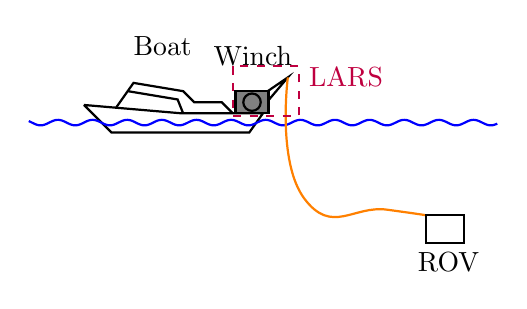
\begin{tikzpicture}[scale=0.7]
    % Boat
    \draw[thick, black] (0,0) -- (.5,-.5) -- (3.,-.5) -- (3.25,-0.15) -- (1.75,-0.15) -- (0,0);
    \draw[thick, black] (0.583,-0.05) -- (0.9,0.4) -- (1.8,0.25) -- (2.,0.05) -- (2.5,0.05) -- (2.7,-0.15);
    \draw[thick, black] (0.8,0.25) -- (1.7,0.1) -- (1.8,-0.15) ;
    \draw[thick, black] (2.75,-0.15) -- (3.7,0.5) -- (3.15,-0.15) ;
    \node[above, xshift=1cm, yshift=0.5cm] {Boat};
    % Surface
    \draw[thick, blue] plot[domain=-1:7.5, samples=300]  (\x,{0.05*sin(\x*10 r)-0.32});
    % Cable
    \draw[thick, orange] plot[smooth, tension=1] coordinates{(3.7,0.5) (4.,-1.7) (5.5, -1.9) (6.2, -2)};
    \filldraw[fill=white, draw=black, thick] (6.2, -2) rectangle (6.9, -2.5) node[below, xshift=-0.2cm] {ROV};
    % LARS
    \draw[thick, purple, dashed] (2.7, 0.7) rectangle (3.9, -0.2) node[right, yshift=0.5cm] {LARS};
    % Winch
    \filldraw[fill=gray, draw=black, thick] (2.75,-0.15) rectangle (3.35,0.25) node[above, xshift=-0.2cm, yshift=0.2cm] {Winch};
    \draw[black, thick] (3.05,0.05) circle (4.5pt);
\end{tikzpicture}